\documentclass[11pt,compress,t,notes=noshow, xcolor=table]{beamer}

\input{../../style/preamble_new}
\input{../../latex-math/basic-math.tex}
\input{../../latex-math/basic-ml.tex}

% ToC
\AtBeginSection[]{
	\begin{frame}[noframenumbering, plain]
	\frametitle{Outline}
	\setcounter{tocdepth}{1}
	\tableofcontents[currentsection]
\end{frame}
}

\title{Deep Learning for NLP II}

\begin{document}

\titlemeta{
Transformer Recap
}{}{
../../slides/chapter03-transformer/figure/transformer_sq.png
}{
\item Understand the scope of the course
\item Answers to all open question
\item Get an impression of the workload
}

% ------------------------------------------------------------------------------

\section{From RNNs to Transformers}

\begin{frame}{Encoder-Decoder RNNs}

\vfill

\begin{tikzpicture}[->, thick, >=stealth]
\node [vec, fill=green!50] (h0) at (0,2) {\scriptsize $\vec h^{(0)}$};
\foreach \i/\word/\coll in {1/a/green,2/great/green,3/book/green,4/!/green,5/BOS/violet,6/ein/violet,7/tolles/violet,8/buch/violet,9/!/violet}{
\node [vec, fill=\coll!50] (x\i) at (\i*1.2, .5) {\scriptsize $\vec x^{(\i)}$};
\node [vec, fill=\coll!50] (h\i) at (\i*1.2, 2) {\scriptsize $\vec h^{(\i)}$};
\draw (x\i) -- (h\i);
\pgfmathparse{\i-1};
\draw (h\pgfmathresult) -- (h\i);
}
\foreach \i/\word/\coll in {1/a/green,2/great/green,3/book/green,4/!/green,5/BOS}{
\node (in\i) [text=black, inner sep=-2pt, outer sep=0pt] at (\i*1.2,-.3) {\scriptsize \phantom{A}\word\phantom{g}};
}

\foreach \i/\word/\coll in {6/ein/violet,7/tolles/violet,8/buch/violet,9/!/violet}{
\node (in\i) [text=red, inner sep=-2pt, outer sep=0pt] at (\i*1.2,-.3) {\scriptsize \phantom{A}\word\phantom{g}};
}

\foreach \i/\word in {5/ein,6/tolles,7/buch,8/!,9/EOS}{
\node (smax\i) [draw, ellipse, inner sep=2pt] at (\i*1.2, 3.5) {\tiny smax};
\node (ffn\i) [draw, ellipse, inner sep=2pt] at (\i*1.2, 2.9) {\tiny lin};
\node (pred\i) [vec] at (\i*1.2, 4.4) {\scriptsize $\vec {\hat{y}}^{(\i)}$};
\node (lab\i) [red] at (\i*1.2, 6.5) {\scriptsize ${y}_\i$};
\node (loss\i) [draw, circle, inner sep=2pt, red] at (\i*1.2, 5.5) {\scriptsize NLL};
\node (out\i) [text=red, inner sep=-2pt] at (\i*1.2,7) {\scriptsize \phantom{A}\word\phantom{g}};
\draw  (h\i) -- (ffn\i);
\draw (ffn\i) -- (smax\i);
\draw  (smax\i) -- (pred\i);
\draw (pred\i) [dashed, red] -- (loss\i);
\draw  (lab\i) [dashed, red] -- (loss\i);
}
\draw [dashed, -] (ffn5)--(ffn6)--(ffn7)--(ffn8)--(ffn9);

\draw [dashed, orange] (0, 4) -- node[midway, above, font=\scriptsize] {inference} (2.3,4);
\draw [orange, draw=none] (0, 4) -- node[midway, below, font=\scriptsize] {(w/ greedy decoding)} (2.3,4);
\draw [dashed, red] (0, 6) -- node[midway, above, font=\scriptsize] {training} (2.3,6);
\draw [red, draw=none] (0, 6) -- node[midway, below, font=\scriptsize] {(w/ oracle inputs)} (2.3,6);

\node [vec, fill=green!50] at (4, 6.4) {\scriptsize encoder};
\node [vec, fill=violet!50] at (4, 4.4) {\scriptsize decoder};

\foreach \j/\t in {6/5,7/6,8/7,9/8}{
\pgfmathparse{\j-1};
\node (argmax\j) [text=orange] at (\j*1.2,-.6) {\scriptsize [?]};
\node [xshift=-1.5mm] (pt\j) at ($(ffn\pgfmathresult)!0.5!(ffn\j)$) {};
\node [xshift=-2.5mm] (px\j) at ($(ffn\pgfmathresult)!0.5!(ffn\j)$) {};
\draw [dashed, red] (out\pgfmathresult) -- (pt\j |- out\pgfmathresult) -- (pt\j |- in\j) -- (in\j);
\draw [dashed, orange] (pred\pgfmathresult) -- (px\j |- pred\pgfmathresult) -- (px\j |- argmax\j) -- (argmax\j);
}
\end{tikzpicture}

\vfill

\end{frame}

% ------------------------------------------------------------------------------

\begin{frame}{Limitations of RNNs}

\vfill

\begin{itemize}
	\item In an RNN, at a given point in time $j$, the information about all past inputs $x^{(1)} \ldots x^{(j)}$ is ``crammed'' into the state vector $\vec h^{(j)}$ (and $\vec c^{(j)}$ for an LSTM)
	\item So for long sequences, the state becomes a \textbf{bottleneck}
	\item Especially problematic in encoder-decoder models (e.g., for Machine Translation)
	\item Solution: Attention \citebutton{Bahdanau et al., 2015 \cite{bahdanau2015neural}}{https://arxiv.org/abs/1409.0473} -- an architectural modification of the RNN encoder-decoder that allows the model to ``attend to'' past encoder states
\end{itemize}

\vfill

\end{frame}

% ------------------------------------------------------------------------------

\begin{frame}{bahdanau attention}
	
\vfill

\begin{figure}
	\centering
		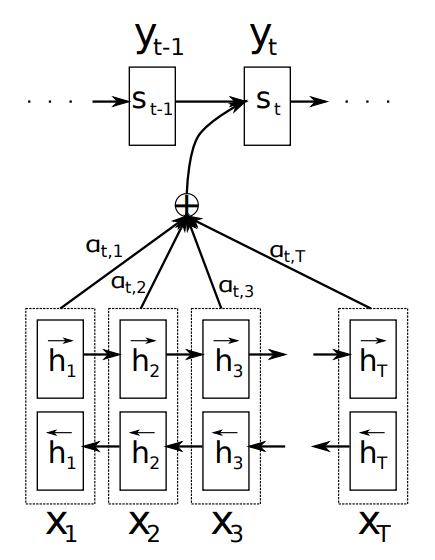
\includegraphics[width = 5.5cm]{../../slides/chapter02-deeplearningbasics/figure/bahdanau-attention.png}\\ 
	\citebutton{Source: Bahdanau et al., 2015 \cite{bahdanau2015neural}}{https://arxiv.org/abs/1409.0473}
\end{figure}

\vfill
	
\end{frame}

% ------------------------------------------------------------------------------

\begin{frame}{modeling long-range dependencies}
	
\vfill

\begin{figure}
	\centering
		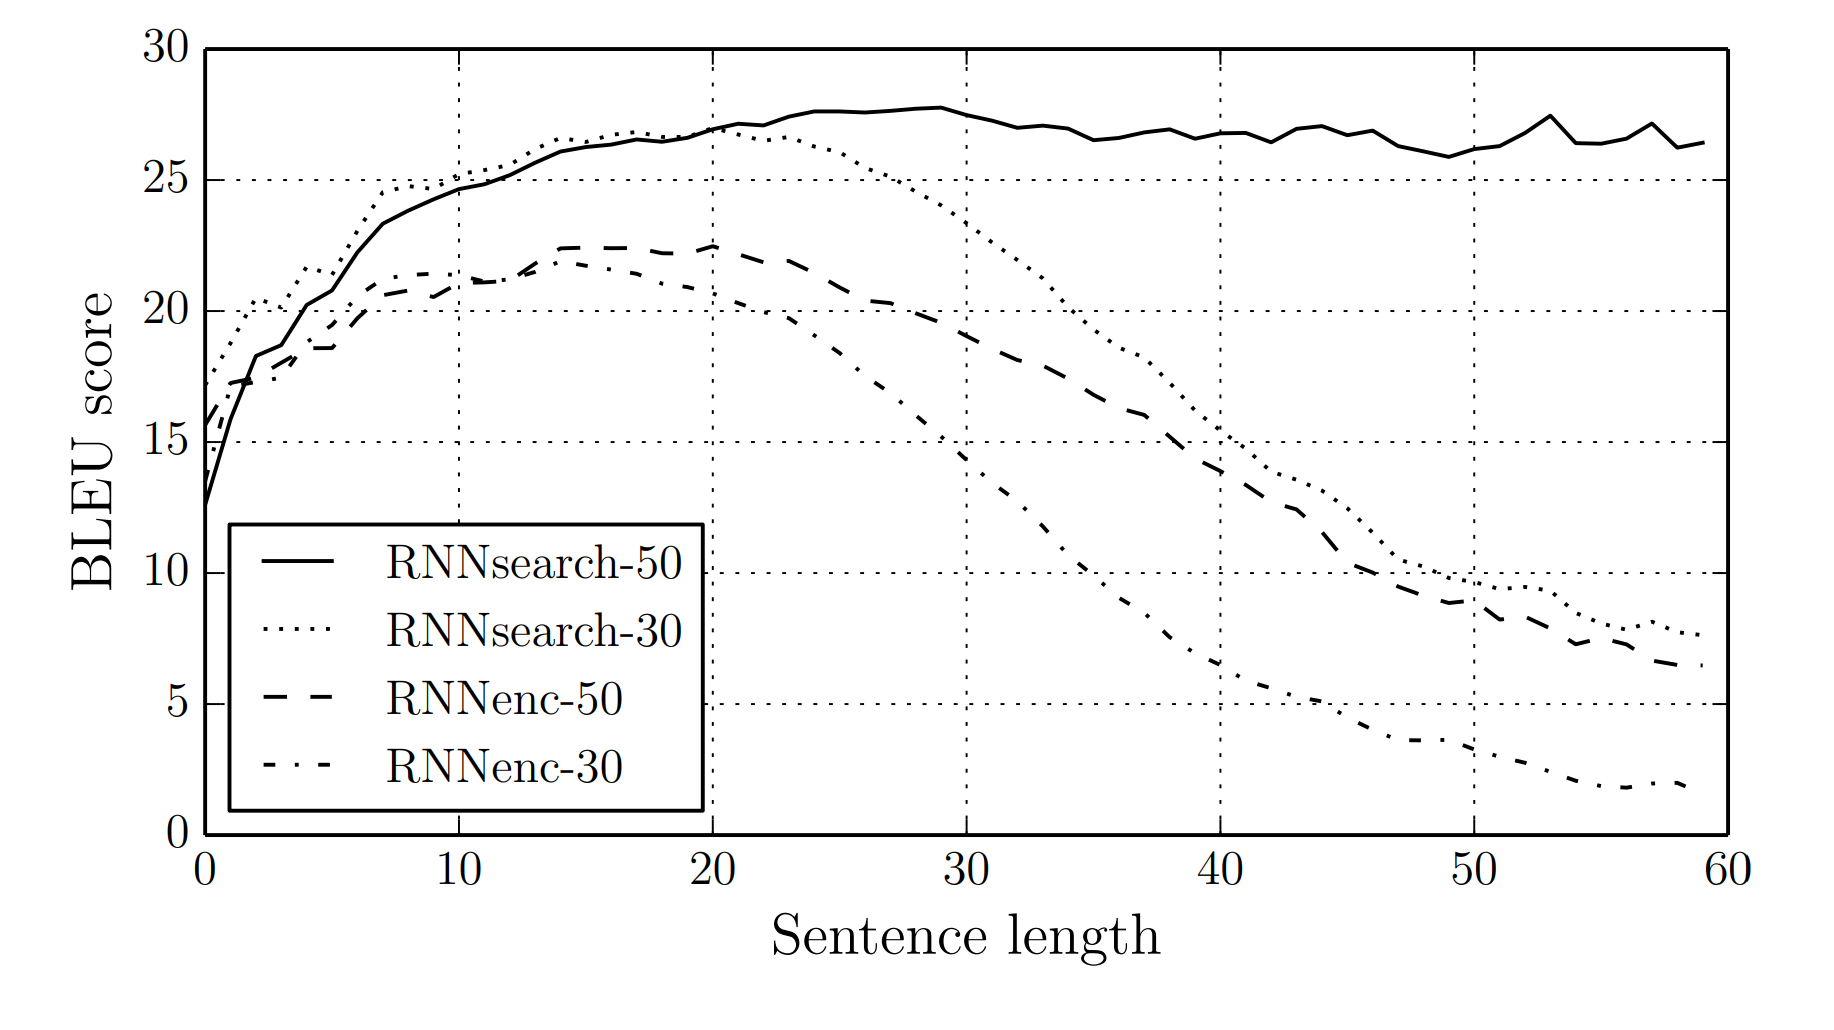
\includegraphics[width = 9cm]{../../slides/chapter02-deeplearningbasics/figure/bahdanau14.png}\\ 
	\citebutton{Source: Bahdanau et al., 2015 \cite{bahdanau2015neural}}{https://arxiv.org/abs/1409.0473}
\end{figure}

\begin{itemize}
	\item RNNenc (classical encoder-decoder); RNNsearch (with Attention)
	\item BLEU score: Measure for translation quality (higher is better)
\end{itemize}

\vfill
	
\end{frame}

% ------------------------------------------------------------------------------

\begin{frame}{Attention: The basic recipe (1)}

\vfill

\textbf{Ingredients:}

\begin{itemize}
	\item One query vector: $\mathbf{q} \in \mathbb{R}^{d_q}$
	\item J key vectors: $\mathbf{K} \in \mathbb{R}^{J \times d_k}; (\vec k_1 \ldots \vec k_J)$
	\item J value vectors: $\mathbf{V} \in \mathbb{R}^{J \times d_v}; (\vec v_1 \ldots \vec v_J)$
	\item Scoring function $a : \mathbb{R}^{d_q} \times \mathbb{R}^{d_k} \rightarrow \mathbb{R}$
		\begin{itemize}
			\item Maps a query-key pair to a scalar (``score'')
			\item May be parametrized by parameters $\theta_a$
		\end{itemize}
\end{itemize}

\vfill

\end{frame}

% ------------------------------------------------------------------------------

\begin{frame}{Attention: The basic recipe (2)}

\vfill

\begin{itemize}
	\item \textbf{Step 1}: Apply $a$ to $\vec q$ and all keys $\vec k_j$ to get scores (one per key): 
	$$\vec e = \begin{bmatrix} e_1 \\ \vdots \\ e_J \end{bmatrix} =  \begin{bmatrix} a(\vec q, \vec k_1; \theta_a) \\ \vdots \\ a(\vec q, \vec k_J; \theta_a) \end{bmatrix}$$
	\item \textbf{Step 2}: Turn $\mathbf{e}$ into a probability distribution with the softmax function
	$$\alpha_j = \frac{\mathrm{exp}(e_j)}{\sum_{j'=1}^J \mathrm{exp}(e_{j'})}$$
		    Note that $\sum_j \alpha_j = 1$

\end{itemize}

\vfill

\end{frame}

% ------------------------------------------------------------------------------

\begin{frame}{Attention: The basic recipe (3)}

\vfill

\begin{itemize}
	\item \textbf{Step 3}: $\alpha$-weighted sum over $\vec {V}$ yields one $d_v$-dimensional output vector:
	$$\vec {o} = \sum_{j=1}^J \alpha_j \vec {v}_j$$
		Intuition: $\alpha_j$ is how much ``attention'' the model pays to $\vec v_j$ when computing $\vec o$.

\end{itemize}

\vfill

\end{frame}

% ------------------------------------------------------------------------------

\begin{frame}{Attention in neural networks}

\vskip-2mm
\vfill

\begin{itemize}
\item \textbf{Important:} $\vec q$, $\vec k_j$ and $\vec v_j$ vectors of a neural network are a function of the input and trainable parameters
\item So the \textit{model} learns which keys are relevant for which queries, based on the training data and loss function
\end{itemize}

\begin{figure}
	\centering
		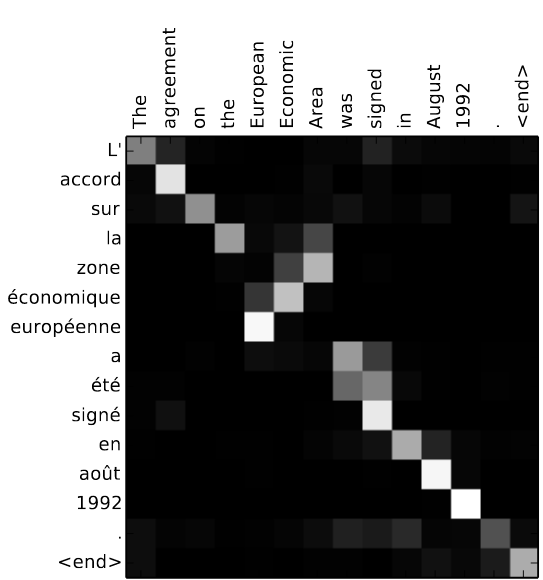
\includegraphics[width = 4.5cm]{../../slides/chapter02-deeplearningbasics/figure/bahdanau4.png}\\ 
	\citebutton{Source: Bahdanau et al., 2015 \cite{bahdanau2015neural}}{https://arxiv.org/abs/1409.0473}
\end{figure}

\vfill

\end{frame}

% ------------------------------------------------------------------------------

\begin{frame}{attention in the transformer (1)}

\vfill

\begin{itemize}
	\item The Bahdanau model is still an RNN, just with attention on top.
	\item Another architecture that consists of attention only: 
		\begin{itemize}
			\item Transformer: ``Attention is all you need'' \citebutton{Vaswani et al., 2017 \cite{vaswani2017attention}}{https://arxiv.org/abs/1706.03762}
			\item No recurrence, \textit{just} Attention (as the name suggests)
			\item Better parallelizable (as opposed to RNNs)
		\end{itemize}
	\item No (or few) assumptions are baked into the architecture (no notion of which words are neighbors in the sentence, sequentiality, etc.)
	\item The lack of prior knowledge often means that the Transformer requires more training data than an RNN to achieve a certain performance
	\item When trained with sufficient data, it usually outperforms them
\end{itemize}

\vfill

\end{frame}

% ------------------------------------------------------------------------------

\begin{frame}{attention in the transformer (2)}

\vfill

\textbf{Cross-Attention:}
    \begin{itemize}
        \item Let $X = (x_1 \ldots x_{J_x}), Y = (y_1 \ldots y_{J_y})$ be two sequences (e.g., source and target in a sequence-to-sequence problem)
        \item The query vectors represent tokens in $Y$ and the key/value vectors represent tokens in $X$ (``$Y$ attends to $X$'')
    \end{itemize}

\medskip\medskip

\textbf{Self-Attention:}
    \begin{itemize}
        \item There is only one sequence $X = (x_1 \ldots x_J)$
        \item The query, key, and value vectors represent tokens in $X$\\
        (``$X$ attends to itself'')
    \end{itemize}

\vfill

\end{frame}

% ------------------------------------------------------------------------------

\begin{frame}{cross-attention vs. self attention}

\vskip-2mm
\begin{tikzpicture}[->, >=stealth]
\foreach \x in {1,2,3}{
\node (x\x) [vec] at (\x, -.5) {$\vec x_\x$};
\node (k\x) [vec] at (\x, 1.5) {$\vec k_\x$};
\node (v\x) [vec] at (\x, 3.5) {$\vec v_\x$};
}
\foreach \y in {1,2}{
\node (y\y) [vec] at (\y+3.5, -.5) {$\vec y_\y$};
\node (q\y) [vec] at (\y+3.5,1.5) {$\vec q_\y$};
\node (o\y) [vec] at (\y+3.5,5.5) {$\vec o_\y$};
\node (alpha\y) [vec, rectangle split, rectangle split parts=3] at (\y+3.5,3.5) {\nodepart{one} $\alpha_{\y,1}$ \nodepart{two} $\alpha_{\y,2}$ \nodepart{three} $\alpha_{\y,3}$};
}

\foreach \y in {1,2}{
\draw (alpha\y.north) -- (o\y.south);
\draw (q\y.north) -- (alpha\y.south);
\draw (y\y.north) -- (q\y.south);
\foreach \x in {1,2,3}{
\draw (v\x.north) -- (o\y.south);
\draw (k\x.north) -- (alpha\y.south);
}}
\foreach \x in {1,2,3}{
\draw (x\x.north) -- (k\x.south);
\draw [bend left=20] (x\x.north west) to (v\x.south west);
}
\node at (3.2, -1.5) {Cross-attention};
\end{tikzpicture}

\end{frame}

% ------------------------------------------------------------------------------

\begin{frame}{cross-attention vs. self attention}

\vskip-2mm
\hfill
\begin{tikzpicture}[->, >=stealth]
\foreach \x in {1,2,3}{
\node (x\x) [vec] at (\x, -.5) {$\vec x_\x$};
\node (k\x) [vec] at (\x, 1.5) {$\vec k_\x$};
\node (v\x) [vec] at (\x, 3.5) {$\vec v_\x$};
}
\foreach \y in {1,2,3}{
\node (q\y) [vec] at (\y+3,1.5) {$\vec q_\y$};
\node (o\y) [vec] at (\y,5.5) {$\vec o_\y$};
\node (alpha\y) [vec, rectangle split, rectangle split parts=3] at (\y+3,3.5) {\nodepart{one} $\alpha_{\y,1}$ \nodepart{two} $\alpha_{\y,2}$ \nodepart{three} $\alpha_{\y,3}$};
}

\foreach \y in {1,2,3}{
\draw (alpha\y.north) -- (o\y.south);
\draw (q\y.north) -- (alpha\y.south);
\draw (x\y.north east) -- (q\y.south west);
\foreach \x in {1,2,3}{
\draw (v\x.north) -- (o\y.south);
\draw (k\x.north) -- (alpha\y.south);
}}
\foreach \x in {1,2,3}{
\draw (x\x.north) -- (k\x.south);
\draw [bend left=20] (x\x.north west) to (v\x.south west);
}
\node at (3.2, -1.5) {Self-attention};
\end{tikzpicture}

\end{frame}

% ------------------------------------------------------------------------------

\begin{frame}{self-attention formalized}

\vfill

\begin{itemize}
\item Let $\vec X \in \mathbb{R}^{J_x \times d_x}$ be a representation of $X$ (e.g., stacked word embeddings, or the outputs of a previous layer)
\item Let $\theta = \{\vec W^{(q)} \in \mathbb{R}^{d_x \times d_q}, \vec W^{(k)} \in \mathbb{R}^{d_x \times d_k}, \vec W^{(v)} \in \mathbb{R}^{d_x \times d_v}\}$\\ be trainable weight matrices
\item We transform $\vec X$ into a matrix of query vectors:
$$ \vec Q = \vec X \vec W^{(q)} $$
\item And we transform $\vec X$ into matrices of key and value vectors:
$$ \vec K = \vec X \vec W^{(k)} ; \qquad \vec V =  \vec X \vec W^{(v)}$$
\item Execute Steps 1 -- 3 of the basic recipe 
\end{itemize}

\vfill

\end{frame}

% ------------------------------------------------------------------------------

\begin{frame}{... as a one-liner}

\vfill

\large
$$ \vec O = \mathcal{F}^\mathrm{attn}(\vec X, \vec X; \theta) = \mathrm{softmax}\Big(\frac{(\vec X\vec W^{(q)} ) (\vec X\vec W^{(k)} )^T}{\sqrt{d_k}}\Big)(\vec X\vec W^{(v)} ) $$
\begin{itemize}
\item GPUs like matrix multiplications\\$\rightarrow$ usually a lot faster than RNN!
\item But: The memory requirements of $\vec E$ and $\vec A$ are $\mathcal{O}(J_x^2)$
\item Sequence lengths are an important issue.
\end{itemize}

\vfill

\end{frame}

% ------------------------------------------------------------------------------

\begin{frame}{Multi-Layer Attention}

\vfill

\begin{itemize}
\item Sequential application of several attention layers, with separate parameters $\{\theta^{(1)} \ldots \theta^{(N)}\}$ 
\item In Transformer: sequential application of Transformer blocks
\item There are some additional position-wise layers inside the Transformer block, i.e., $\vec O^{(n)}$ undergoes some additional transformations before becoming the input to the next Transformer block $n+1$
\end{itemize}

\vfill

\end{frame}

% ------------------------------------------------------------------------------

\begin{frame}{Multi-Head Attention}

\vfill

\begin{itemize}
\item Application of several attention layers (``heads'') in parallel
\item $M$ sets of parameters $\{\theta^{(1)}, \ldots, \theta^{(M)}\}$, with $\theta^{(m)} = \{\vec {W}^{(m,q)}, \vec {W}^{(m,k)}, \vec {W}^{(m,v)}\}$
\item For every head, compute in parallel:
$$ \vec O^{(m)} = \mathcal{F}^\mathrm{attn}(\vec X, \vec Y; \theta^{(m)}) $$
\item Choice of dimensionality: $d_k = d_v = d_{x}/M$ 
\item Concatenate all $\vec {O}^{(m)}$ along their last axis; then down-project the concatenation with an additional parameter matrix $\vec W^{(o)} \in \mathbb{R}^{Md_v \times d_v}$:
$$ \vec O = [\vec O^{(1)}; \ldots;  \vec O^{(M)}] \vec W^{(o)}$$
\end{itemize}

\vfill

\end{frame}

% ------------------------------------------------------------------------------

\section{Positional Information}

\begin{frame}{Can self-attention model word order?}

\vfill

\begin{itemize}
	\item Hypothetical model:
			\begin{itemize}
				\item simple word embedding lookup layer
				\item self-attention layer 
				%\item (For simplicity, we only consider one head, but this applies to multi-head attention as well.)
			\end{itemize}
	\item Let $\blu{X^{(1)}}$, $\org{X^{(2)}}$ be two sentences of the same length $J$, which contain the same words, but in a different order
	\item Example: \blu{``john loves mary''} vs. \org{``mary loves john''}
\end{itemize}
\begin{center}
	
\includegraphics[width=.5\textwidth]{../../slides/chapter03-transformer/figure/mary_loves_john.png}
\end{center}

\begin{itemize}
\item But: The representation of \blu{mary} is identical to that of \org{mary}, and the representation of \blu{john} is identical to that of \org{john}
\end{itemize}
\vfill

\end{frame}

% ------------------------------------------------------------------------------

\begin{frame}{Position embeddings}

\vfill

\begin{itemize}
\item Self-attention computes each output as a \textit{weighted sum of all inputs}
\item The weights depend only on content -- not on the order of tokens
\item Self-attention is therefore \textbf{permutation-equivariant}:
\end{itemize}

\begin{equation*}
\text{Attn}(\pi(\vec x_1, \ldots, \vec x_n)) = \pi\big(\text{Attn}(\vec x_1, \ldots, \vec x_n)\big)
\quad \forall\, \text{permutations } \pi
\end{equation*}

\begin{itemize}
\item Add to every input word embedding a position embedding $\vec {p} \in \mathbb{R}^d$:
\item Input embedding of word ``mary'' in position $j$: $\vec {x}_j = \vec {w}_{\mathcal{I}(\text{mary})} + \mathbf{p}_j$
$$\vec {w}_{\mathcal{I}(\text{mary})} + \vec {p}_j \neq \vec{w}_{\mathcal{I}(\text{mary})} + \vec {p}_{j'} \text{ if } j \neq j'$$

\end{itemize}

\vfill

\end{frame}

% ------------------------------------------------------------------------------

\begin{frame}{Absolute Positional Encodings}

\vfill

\begin{itemize}
\item Option 1 (fixed) \citebutton{Vaswani et al., 2017 \cite{vaswani2017attention}}{https://arxiv.org/abs/1706.03762}\\ 
(Deterministic) Sinusoidal position embeddings: 
$$p_{j,i} = \begin{cases} \mathrm{sin}\big(\frac{j}{10000^\frac{i}{d}}\big)  & \text{ if } i \text{ is even} \\ \mathrm{cos}\big(\frac{j}{10000^\frac{i-1}{d}}\big) & \text{ if } i \text{ is odd}  \end{cases}$$
\item Option 2 (learned) \citebutton{Source: Devlin et al., 2019 \cite{devlin-etal-2019-bert}}{https://aclanthology.org/N19-1423.pdf}\\
Trainable position embeddings: $\vec {P} \in \mathbb{R}^{J^\mathrm{max} \times d}$\\
(Disadvantage: Cannot deal with sentences longer than $J^\mathrm{max}$)
\end{itemize}

\vfill

\end{frame}

% ------------------------------------------------------------------------------

\begin{frame}{Relative Positional Encodings}

\vfill

\begin{itemize}
\item Key idea: inject relative offset $(i-j)$ directly into the attention computation
\citebutton{Shaw et al. (2018) \cite{shaw-etal-2018-self}}{https://aclanthology.org/N18-2074/}
\item Learnable per-offset vectors $\vec a^K_{i-j}$ and $\vec a^V_{i-j}$ augment keys and values:
\end{itemize}

\begin{equation*}
e_{i,j} = \frac{(\vec x_i\rmW^Q)\bigl(\vec x_j\rmW^K + \vec a^{K}_{i-j}\bigr)^\top}{\sqrt{d_k}},
\qquad
\vec o_i = \sum_j \alpha_{i,j}\bigl(\vec x_j\rmW^V + \vec a^{V}_{i-j}\bigr)
\end{equation*}

\begin{itemize}
\item The model now conditions \textit{directly} on relative distance when computing each attention weight
\item Offsets are clipped to $[-k, k]$ to keep the learnable table finite: $\vec a^K_{\max(-k,\,\min(k,\,i-j))}$
\item Requires $O(n^2)$ additional terms -- memory overhead for long sequences
\end{itemize}

\vfill

\end{frame}

% ------------------------------------------------------------------------------

\begin{frame}{Attention with Linear Biases}

\vfill

\begin{itemize}
\item Completely removes position embeddings; instead adds a \textit{fixed} scalar bias to each attention logit
\citebutton{ALiBi (Press et al., 2022) \cite{press2022train}}{https://openreview.net/forum?id=R8sQPpGCv0}
\item The bias penalizes attention to distant tokens proportionally to their distance:
\end{itemize}

\begin{equation*}
e_{i,j} = \frac{\vec q_i^\top \vec k_j}{\sqrt{d_k}} - m_h \cdot |i - j|
\end{equation*}

\begin{itemize}
\item Slope $m_h$ is head-specific and \textit{fixed}\\(geometric sequence: $\frac{1}{2^1}, \frac{1}{2^2}, \ldots, \frac{1}{2^H}$)
\item No position vectors added to inputs; no extra parameters to train
\item Strong length-extrapolation: trained on 1024 tokens, generalizes well to 2048+
\item Used in MPT, BLOOM, and other large open-weight LLMs
\end{itemize}

\vfill

\end{frame}

% ------------------------------------------------------------------------------

\begin{frame}{Rotary Positional Embeddings}

\vfill

\begin{itemize}
\item RoPE encodes position by \textit{rotating} query/key vectors in consecutive 2D subspaces
\citebutton{Su et al. (2021) \cite{SU2024127063}}{https://doi.org/10.1016/j.neucom.2023.127063}
\item For each pair of dimensions $(2m, 2m+1)$, apply a rotation by angle $j \cdot \theta_m$:
\end{itemize}

\begin{equation*}
\theta_m = \text{base}^{-2m/d}, \quad \text{base} = 10000
\end{equation*}

{\footnotesize
$$
\mathrm{RoPE}(\vec q, j) = \mathbf{R}(j)\vec q,
$$\\
$$
\mathbf{R}(j) = \mathrm{diag}\!\left(
\begin{bmatrix}\cos j\theta_0 & -\sin j\theta_0 \\ \sin j\theta_0 & \cos j\theta_0\end{bmatrix},
\;\ldots,\;
\begin{bmatrix}\cos j\theta_{d/2-1} & -\sin j\theta_{d/2-1} \\ \sin j\theta_{d/2-1} & \cos j\theta_{d/2-1}\end{bmatrix}
\right)
$$
} 

\begin{itemize}
\item Applied to $\vec q$ and $\vec k$ only -- no change to values or embeddings
\end{itemize}

\vfill

\end{frame}

% ------------------------------------------------------------------------------

\section{Autoregressive Models}

\begin{frame}{RNNs for autoregressive LM \& decoding}

\vfill

\begin{itemize}
\item In autoregressive language modeling, or in the decoder of a sequence-to-sequence model, the task is to always predict the next word
\item In an RNN, a given state $\vec h^{(j)}$ depends on past inputs $x^{(1)} \ldots x^{(j)}$
\item Thus, the RNN is unable to ``cheat'':
\end{itemize}
\begin{center}
\begin{tikzpicture}
\node (h0) [vec, minimum height=7mm] at (0, 1) {$\vec h^{(0)}$};
\foreach \i/\word in {1/BOS,2/a,3/great,4/book,5/!}{
\node (h\i) [vec, minimum height=7mm] at (\i*1.5, 1) {$\vec h^{(\i)}$};
\node (yhat\i) [vec, minimum height=7mm] at (\i*1.5, 2) {$\vec {\hat{y}}^{(\i)}$};
\node (nll\i) [draw, circle, inner sep=2pt] at (\i*1.5, 3) {\scriptsize $NLL$};
\node (e\i) [vec, minimum height=7mm] at (\i*1.5, 0) {$\vec x^{(\i)}$};
}
\foreach \i/\word in {1/BOS,2/a,3/great,4/book,5/!}{
\node (w\i) [font=\scriptsize, inner sep=0] at (\i*1.5, -.7) {\phantom{A}\word\phantom{g}};
}

\foreach \i/\word in {1/a,2/great,3/book,4/!, 5/EOS}{
\node (y\i) [font=\scriptsize, inner sep=0] at (\i*1.5, 3.8) {\phantom{A}\word\phantom{g}};
}

\foreach \i/\j in {0/1, 1/2, 2/3, 3/4, 4/5}{
\draw [->, >=stealth, thick] (h\i) -- (h\j);
\draw [->, >=stealth, thick] (e\j) -- (h\j);
\draw [->, >=stealth, thick] (h\j) -- (yhat\j);
\draw [->, >=stealth, thick] (yhat\j) -- (nll\j);
\draw [->, >=stealth, thick] (y\j) -- (nll\j);
} 
\foreach \i/\j in {1/2, 2/3, 3/4, 4/5}{
\node at ($(h\i)!0.5!(h\j)$) [inner sep=0pt] (p) {};
\draw [->, >=stealth, thick, dashed] (y\i.east)  --(p|-y\i.east) -- (p) -- (p |- w\j.west) -- (w\j.west);
}
\end{tikzpicture}
\end{center}
\vfill

\end{frame}

% ------------------------------------------------------------------------------

\begin{frame}{Self-attention for AR LM \& decoding}

\begin{itemize}
\item With attention, all $\vec o_j$ depend on all $\vec v_{j'}$ (and by extension, all $\vec x_{j'}$).
\item This means that the model can easily cheat by looking at future words (red connections)
\end{itemize}
\begin{center}
\begin{tikzpicture}
\foreach \i/\word in {1/BOS,2/a,3/great,4/book,5/!}{
\node (h\i) [vec, minimum height=7mm] at (\i*1.5, 1) {$\vec o_\i$};
\node (yhat\i) [vec, minimum height=7mm] at (\i*1.5, 2) {$\vec {\hat{y}}_\i$};
\node (nll\i) [draw, circle, inner sep=2pt] at (\i*1.5, 3) {\scriptsize $NLL$};
\node (e\i) [vec, minimum height=7mm] at (\i*1.5, -.5) {$\vec v_\i$};
\node (x\i) [vec, minimum height=7mm] at (\i*1.5, -1.5) {$\vec x_\i$};
}
\foreach \i/\word in {1/BOS,2/a,3/great,4/book,5/!}{
\node (w\i) [font=\scriptsize, inner sep=0] at (\i*1.5, -2.1) {\phantom{A}\word\phantom{g}};
}

\foreach \i/\word in {1/a,2/great,3/book,4/!, 5/EOS}{
\node (y\i) [font=\scriptsize, inner sep=0] at (\i*1.5, 3.7) {\phantom{A}\word\phantom{g}};
}

\foreach \i/\j in {0/1, 1/2, 2/3, 3/4, 4/5}{
\draw [->, >=stealth, thick] (h\j) -- (yhat\j);
\draw [->, >=stealth, thick] (yhat\j) -- (nll\j);
\draw [->, >=stealth, thick] (y\j) -- (nll\j);
\draw [->, >=stealth, thick] (x\j) -- (e\j);
} 
\foreach \i in {1,2,3,4,5}{
\foreach \j in {\i,...,5}{
\draw [<-, >=stealth, red] (h\i.south) -- (e\j.north);
}
\foreach \i in {1,2,3,4,5}{
\foreach \j in {\i,...,5}{
\draw [->, >=stealth, green] (e\i.north) -- (h\j.south);
}
}
}

\foreach \i/\j in {1/2, 2/3, 3/4, 4/5}{
\node at ($(h\i)!0.5!(h\j)$) [inner sep=0pt] (p) {};
\draw [->, >=stealth, thick, dashed] (y\i.east)  --(p|-y\i.east) -- (p) -- (p |- w\j.west) -- (w\j.west);
}
\end{tikzpicture}
\end{center}

\end{frame}

% ------------------------------------------------------------------------------

\begin{frame}{Parallelized masked self-attention}

\vfill

\begin{itemize}
\item Step 1: Calculate $\vec E$ like we usually would
\item Step 1B:
$$
\begin{aligned}
\vec E^\mathrm{masked} & = \vec E \odot \vec M + \infty\vec M-\infty; \qquad m_{j,j'} = \begin{cases} 1 & \text{ if } j' \leq j \\ 0 & \text{ otherwise} \end{cases}
\end{aligned}
$$
\item Example:
\end{itemize}
$$
\begin{aligned}
\vec E & = \begin{bmatrix} e_{1,1} & e_{1,2} & e_{1,3} \\ e_{2,1} & e_{2,2} & e_{2,3} \\ e_{3,1} & e_{3,2} & e_{3,3} \end{bmatrix}; \qquad \vec M = \begin{bmatrix} 1 & 0 & 0 \\ 1 & 1 & 0 \\ 1 & 1 & 1 \end{bmatrix} \\
\vec E^\mathrm{masked} & = \begin{bmatrix} e_{1,1} & -\infty & -\infty \\ e_{2,1} & e_{2,2} & -\infty \\ e_{3,1} & e_{3,2} & e_{3,3} \end{bmatrix} ; \qquad \vec A^\mathrm{masked} = \begin{bmatrix} 1 & 0 & 0 \\ \alpha_{2,1} & \alpha_{2,2} & 0 \\ \alpha_{3,1} & \alpha_{3,2} & \alpha_{3,3} \end{bmatrix} \\
\vec o_1 = \vec v_1; \qquad & \vec o_2 = \alpha_{2,1} \vec v_1 + \alpha_{2,2} \vec v_2; \qquad \vec o_3 = \alpha_{3,1} \vec v_1 + \alpha_{3,2} \vec v_2 + \alpha_{3,3} \vec v_3
\end{aligned}
$$

\vfill

\end{frame}

% ------------------------------------------------------------------------------

\begin{frame}{AR Transformer at inference time}

\vfill

\begin{itemize}
\item During training (targets known): Use parallelized masked attention 
\item At inference time (targets unknown): Decode prediction in a loop
\item Slower, but at least we don't have to worry about masking anymore
\end{itemize}
\begin{center}
\begin{tikzpicture}
\foreach \i/\word in {1/BOS,2/a,3/great,4/book,5/!}{
\node (h\i) [vec, minimum height=7mm] at (\i*1.5, 1) {$\vec o_\i$};
\node (yhat\i) [vec, minimum height=7mm] at (\i*1.5, 2) {$\vec {\hat{y}}_\i$};
\node (e\i) [vec, minimum height=7mm] at (\i*1.5, -.5) {$\vec v_\i$};
\node (x\i) [vec, minimum height=7mm] at (\i*1.5, -1.5) {$\vec x_\i$};
}
\foreach \i/\word in {2/a,3/great,4/book,5/!}{
\node (w\i) [font=\scriptsize, inner sep=0, orange] at (\i*1.5, -2.1) {[?]};
}
\foreach \i/\word in {1/BOS}{
\node (w\i) [font=\scriptsize, inner sep=0] at (\i*1.5, -2.1) {BOS};
}

\foreach \i/\j in {0/1, 1/2, 2/3, 3/4, 4/5}{
\draw [->, >=stealth, thick] (h\j) -- (yhat\j);
\draw [->, >=stealth, thick] (x\j) -- (e\j);
} 
\foreach \i in {1,2,3,4,5}{
\foreach \j in {\i,...,5}{
\draw [->, >=stealth, green] (e\i.north) -- (h\j.south);
}
}

\foreach \i/\j in {1/2, 2/3, 3/4, 4/5}{
\node at ($(h\i)!0.5!(h\j)$) [inner sep=0pt] (p) {};
\draw [->, >=stealth, thick, dashed, orange] (yhat\i.east)  --(p|-yhat\i.east) -- (p) -- (p |- w\j.west) -- (w\j.west);
\node at ([xshift=2mm, yshift=5mm] yhat\i.east) [rotate=90, font=\tiny, orange] {argmax};
}
\end{tikzpicture}
\end{center}

\vfill

\end{frame}


% ------------------------------------------------------------------------------

\begin{frame}{The Transformer architecture}

\begin{center}
\begin{tikzpicture}[->, >=stealth, thick, font=\scriptsize]
\node (transformer) at (0,0) {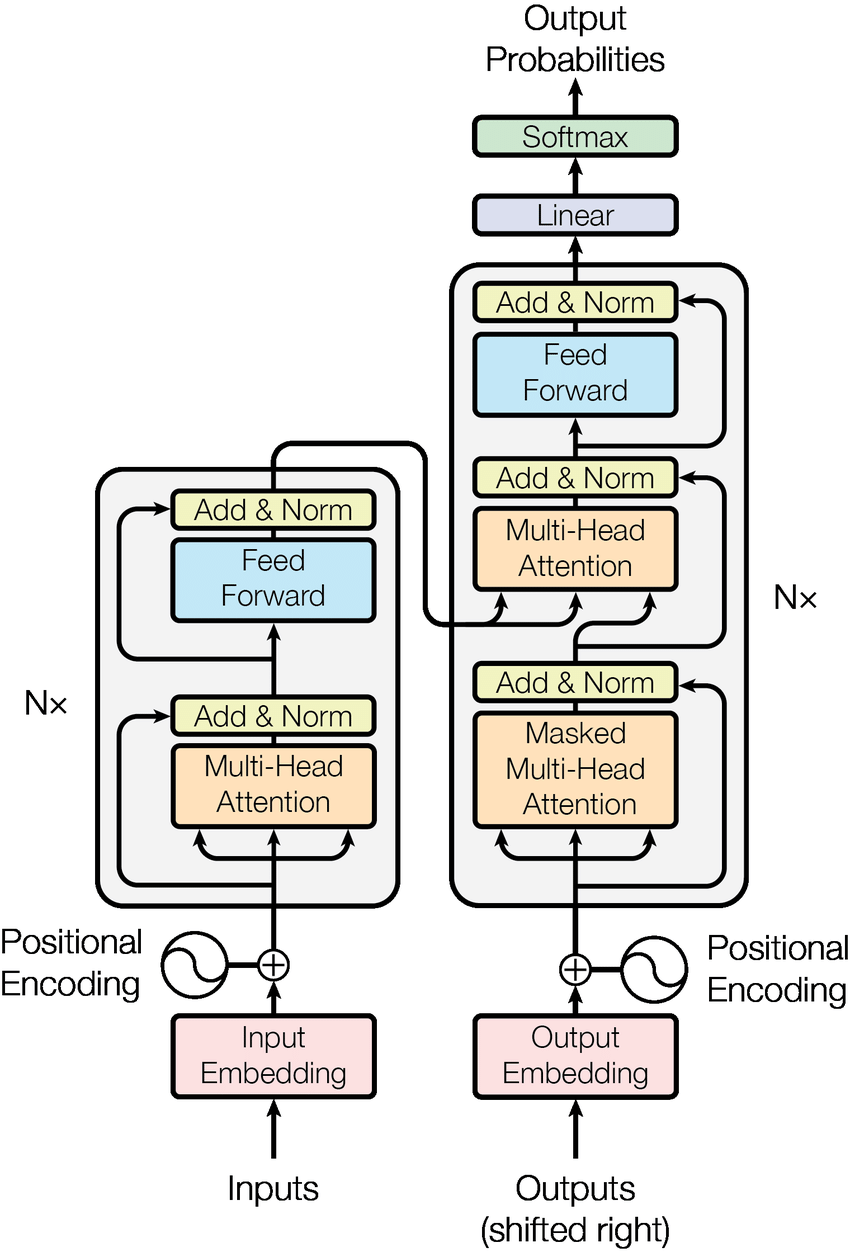
\includegraphics[width=.4\textwidth]{../../slides/chapter03-transformer/figure/transformer.png}};
\node (enc) [left=2mm of transformer, rotate=90] {encoder};
\node (dec) [right=2mm of transformer, rotate=270] {decoder};
\node (x) [above left=1cm of transformer.south west] {$X$ (source)};
\node (y) [above right=1cm of transformer.south east] {$Y$ (target)};
\draw (x) -- ([yshift=5mm, xshift=1cm] transformer.south west);
\draw (y) -- ([yshift=5mm, xshift=-1cm] transformer.south east);
\node (nll) [draw, circle] at ([yshift=-5mm] transformer.north east) {NLL};
\draw [bend right=55] (y.north east) to (nll);
\draw ([xshift=-1cm, yshift=-5mm] transformer.north east) to (nll);
\node at (-3, 2) [align=left] {(For simpler problems (e.g., \\ classification, tagging), \\ you would simply use \\ the encoder.)};
\end{tikzpicture}\\ 
	\citebutton{Source: Vaswani et al., 2017 \cite{vaswani2017attention}}{https://arxiv.org/abs/1706.03762}
\end{center}

\end{frame}

% ------------------------------------------------------------------------------

\begin{frame}{Why do we care about the Parameter Count?}
\begin{itemize}
    \item Being able to derive the parameter count of a model requires good knowledge of the math behind the model architecture
    \item So by deriving the parameter count, we learn how the model works under the hood
    \item Since models just stack various building blocks on top of each other, we can reuse the derived parameter count for all sorts of models
    \item We get an idea about how the parameters scale with increasing model size
\end{itemize}
\end{frame}

% ------------------------------------------------------------------------------

\section{Parameter Counts}

\begin{frame}{Overview over Parameter Sources}
\vfill
\begin{minipage}[c]{.49\textwidth}
    \vfill
    \begin{figure}
		\centering
		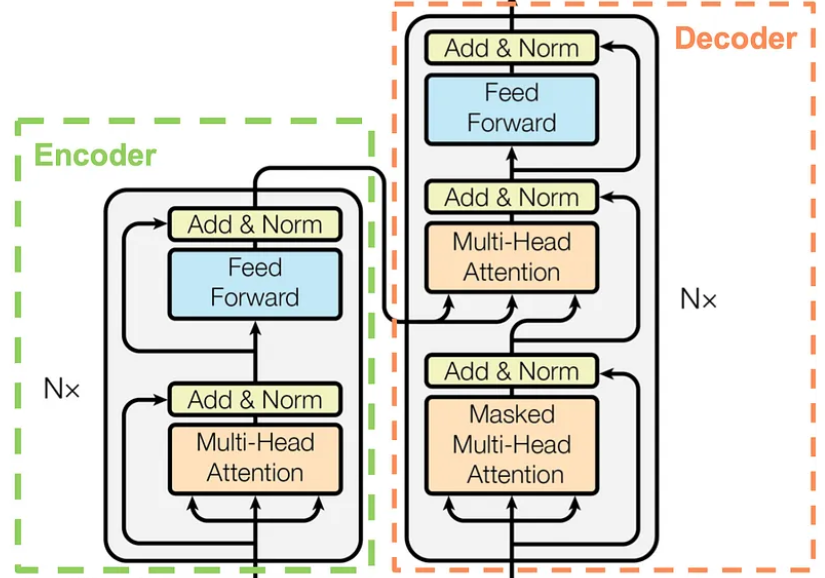
\includegraphics[]{../../slides/chapter03-transformer/figure/enc_dec.png}
	\end{figure}
    \vfill
\end{minipage}
\hfill
\begin{minipage}[c]{.49\textwidth}
    \hfill
    \begin{itemize}
        \item \textbf{Encoder}
        \begin{itemize}
            \item Multi-Head Attention
            \item 2x Layernorm
            \item Feed Forward Network
        \end{itemize}
        \item \textbf{Decoder}
        \begin{itemize}
            \item 2x Multi-Head Attention
            \item 3x Layernorm
            \item Feed Forward Network
        \end{itemize}
    \end{itemize}
\end{minipage}
\vfill
\textit{So all we have to do is to derive the parameter count of each of those components and then sum them up!} \citebutton{Vaswani et al., 2017}{https://arxiv.org/abs/1706.03762}

\end{frame}

%-------------------------------------------------------------------------------

\begin{frame}{Multi Head Attention (1)}

\begin{minipage}[c]{.44\textwidth}
    \vfill
    \begin{figure}
        \centering
        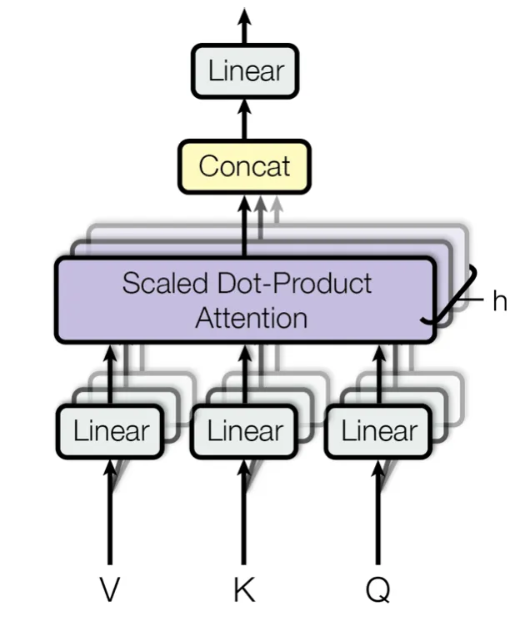
\includegraphics{../../slides/chapter03-transformer/figure/mha.png}
        \label{fig:enter-label}
    \end{figure}
    \vfill
\end{minipage}
\hfill
\begin{minipage}[c]{.54\textwidth}
    \begin{itemize}
        \item The input token embeddings have shape $d_{model}$ (embedding dimension)
        \item Project input embeddings into Query, Keys and Values with matrices $\boldsymbol{W_Q}$, $\boldsymbol{W_K}$, $\boldsymbol{W_V}$ for each head (so we have $n_{head}$ ($h$ in the image) of each Matrix)
        \item Project concatenated output of the Scaled Dot-Product Attention back to $d_{model}$ with $\boldsymbol{W_O}$
    \end{itemize}
\end{minipage}
\vfill
\textit{To get to the total parameter count, we simply have to calculate the number of parameters in all of those Matrices! (for now, we also include the bias terms of the linear projections)}

    
\end{frame}

%-------------------------------------------------------------------------------

\begin{frame}{Multi Head Attention (2)}

\begin{itemize}
    \item \textbf{Project Input Sequence into Query, Key and Value:}
        \begin{itemize}
            \item Input shape: $seq\_len\times d_{model}$ ($seq\_len$ is the number of tokens, where each has the embedding dimension of $d_{model}$)
            \item For MHA we project $d_{model}$ to $d_{qkv}$, with $d_{qkv} = d_{model}/n_{head}$ \item We split up $d_{model}$ into $n_{head}$ heads and need $\boldsymbol{W_Q}$, $\boldsymbol{W_K}$, $\boldsymbol{W_V}$ for each head
            \item Each Matrix has shape $d_{model} \times d_{qkv}$
        \end{itemize}
    \vfill
    \item \textbf{Project concatenated output to the MHA output:}
        \begin{itemize}
            \item We concatenate the $n_{head}$ outputs, where each has shape $d_{qkv}$ and end up with a shape of $d_{model}$ again
            \item We then project $d_{model}$ to $d_{model}$ with $\boldsymbol{W_O}$
            \item $\boldsymbol{W_O}$ thus has a shape of $d_{model} \times d_{model}$
        \end{itemize}
\end{itemize}
    
\end{frame}

%-------------------------------------------------------------------------------

\begin{frame}{Multi Head Attention (3)}

\textit{Now we put both parts together:}

$$
\begin{aligned}
N_{attention} &= \underbrace{(d_{model} \times d_{model} + d_{model})}_{W_O} \\
&\quad + \underbrace{(d_{model} \times d_{qkv} + d_{qkv})}_{W_{Q,K,V}} \times \overbrace{n_{heads} \times 3}^{\text{3 matrices for each head}} \\
&= (d_{model} \times d_{model} + d_{model}) + (d_{model} \times d_{model} + d_{model}) \times 3 \\
&= \underbrace{(d_{model}^2 + d_{model}) \times 4}_{\text{The exact formula}} \\
&\approx \underbrace{4 \cdot d_{model}^2}_{\text{Approximation}}
\end{aligned}
$$

\end{frame}


%-------------------------------------------------------------------------------

\begin{frame}{Feed Forward Network}
    \begin{itemize}
        \item The FFN of the Transformer uses two fully connected layers
        \item Input and output size is both $d_{model}$
        \item The hidden layer size is $4 \times d_{model}$ (\textit{This is a decision by the authors of the paper!)}
        \item Our weight matrices $W_1$ and $W_2$ therefore have shape $d_{model} \times 4\cdot d_{model}$ and $4\cdot d_{model} \times d_{model}$ respectively
    \end{itemize}
    
    \begin{align*}
    N_{FFN} &= (d_{model} \times 4\cdot d_{model} +4\cdot d_{model}) + (4\cdot d_{model} \times d_{model} + d_{model}) \\
    &= 8\cdot d_{model}^2 + 5\cdot d_{model} \\
    &\approx 8\cdot d_{model}^2    
    \end{align*}
\end{frame}

%-------------------------------------------------------------------------------

\begin{frame}{Layer Norm}

\begin{itemize}
    \item We estimate $\mu$ and $\sigma$ for each layer (\textit{H denotes the number of hidden neurons in a layer}):
\end{itemize}
$$\mu = \frac{1}{N} \sum^{H}_{i=1}a_{i}$$
$$\sigma = \sqrt{\frac{1}{N} \sum^{H}_{i=1}{(a_{i}-\mu})^2}$$

\begin{itemize}
    \item For rescaling the normalizations we need a $\beta$ and $\gamma$ parameter for each neuron in the layer
    \item Since our layer has $d_{model}$ neurons we need $2\cdot d_{model}$ parameters for the Layer Norm operations
\end{itemize}

$$N_{Layernorm} = 2\cdot d_{model}$$
    
\end{frame}
%-------------------------------------------------------------------------------

\begin{frame}{Exact Parameter Count}
\textit{All we have to do now is to sum up the Parameter counts of each component for both the Encoder and Decoder!}

\begin{align*}
N_{Encoder} &= 1\cdot N_{attention} + 1\cdot N_{FFN} + 2\cdot N_{Layernorm} \\
&= 4\cdot(d_{model}^2 + d_{model}) + 8\cdot d_{model}^2 + 5\cdot d_{model} + 2\cdot(2\cdot d_{model}) \\
&= 12\cdot d_{model}^2 + 13 \cdot d_{model}
\end{align*}

\vspace{-.5cm}

\begin{align*}
N_{Decoder} &= 2\cdot N_{attention} + 1\cdot N_{FFN} + 3\cdot N_{Layernorm}\\
&= 2\cdot 4\cdot (d_{model}^2 + d_{model}) + 8\cdot d_{model}^2 + 5\cdot d_{model} + 3\cdot (2\cdot d_{model}) \\
&= 16\cdot d_{model}^2 + 19\cdot d_{model}
\end{align*}

\vspace{-.5cm}

\begin{align*}
N_{Total} &= 12\cdot d_{model}^2 + 13\cdot d_{model} + 16\cdot d_{model}^2 + 19\cdot d_{model} \\
&= 28\cdot d_{model}^2 + 29\cdot d_{model}
\end{align*}


\end{frame}
%-------------------------------------------------------------------------------

\begin{frame}{Approximate Parameter Count}

\textit{Since the parameter count scales quadratically with $d_{model}$ we can approximate it by omitting the layernorm parameters and the bias terms!} 
$$N_{Encoder} = 1\cdot N_{attention} + 1\cdot N_{FFN} = 4\cdot d_{model}^2 + 8\cdot d_{model}^2 = 12 \cdot d_{model}^2$$

$$N_{Decoder} = 2\cdot N_{attention} + 1\cdot N_{FFN} = 2\cdot 4\cdot d_{model}^2 + 8\cdot d_{model}^2 = 16\cdot d_{model}^2$$

$$N_{Total} = 12\cdot d_{model}^2 + 16\cdot d_{model}^2 = 28\cdot d_{model}^2$$
\vfill
\textit{This is the approximate parameter count for one layer!}

\end{frame}

%-------------------------------------------------------------------------------

\begin{frame}{Calculate parameter count}
\textit{Now we can calculate the parameter count of the vanilla transformer}

\begin{itemize}
    \item From the paper we know $n_{Layers} = 6$ for both Encoder and Decoder and $d_{model} = 512$
    \item Let's first use the exact formula:

\begin{align*}
N_{Params} &= 6\cdot(12\cdot 512^2 + 13\cdot 512) + 6\cdot(16\cdot 512^2 + 19\cdot 512) \\
&= 44,138,496
\end{align*}

    \item And now with the approximation:

\begin{align*}
N_{Params} &= 6\cdot(12\cdot 512^2) + 6\cdot(16\cdot 512^2) \\
&= 44,040,192
\end{align*}

\end{itemize}

\textit{The approximation is really good, which is why we can ignore the bias and layernorm parameters!}
    
\end{frame}

%-------------------------------------------------------------------------------

\begin{frame}{Embedding Parameters}
    \textit{We also have to consider the parameters of the embeddings:}
    \vspace{1em}
    \begin{itemize}
        \item Let $M$ be the maximum sequence length and $V$ the size of the vocabulary
        \item We have $M \times d_{model}$ positional embedding parameters, which are fixed and not learned
        \item And $V \times d_{model}$ token embeddings parameters, which are learned
        \item The original transformer has $V = 37000$ tokens:
    			$$N_{Embedding} = 37000 \cdot 512 = 18,944,000$$
    		\item Adding those to the previous count yields:
    			$$N_{Final} = 18,944,000 + 44,040,192 = 62,984,192$$     
    \end{itemize}
\end{frame}

% ==============================================================================

\begin{frame}[allowframebreaks,noframenumbering,plain]{References}
        \tiny
        \bibliographystyle{plain} %apalike
        \bibliography{../../anthology-1,../../anthology-2,intro}
\end{frame}

\endlecture
\end{document}